\chapter{Test}
\todo[inline]{Remember photos of the different test setups!}
The order of the test is defined from which tests that can harm the system. The most destructive tests are taken in the end. 
The test procedure 
\section{Radiation test}
The test is performed in a TEM-cell (Transverse ElectroMagnetic field cell).
The measurement in a TEM-cell can be compared to an open air measurement if the object is small and without inlets. 

\begin{figure}[H]
	\begin{centering}
		 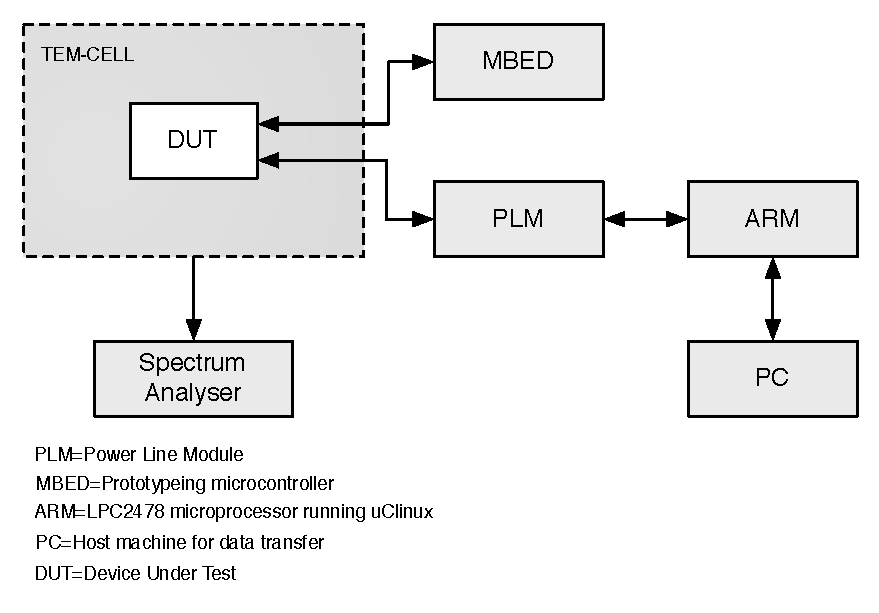
\includegraphics[width=0.8\textwidth]{images/emission_setup.pdf}
		\caption{Emission test setup.}
	\end{centering}
\end{figure}

\begin{figure}[H]
	\begin{centering}
		 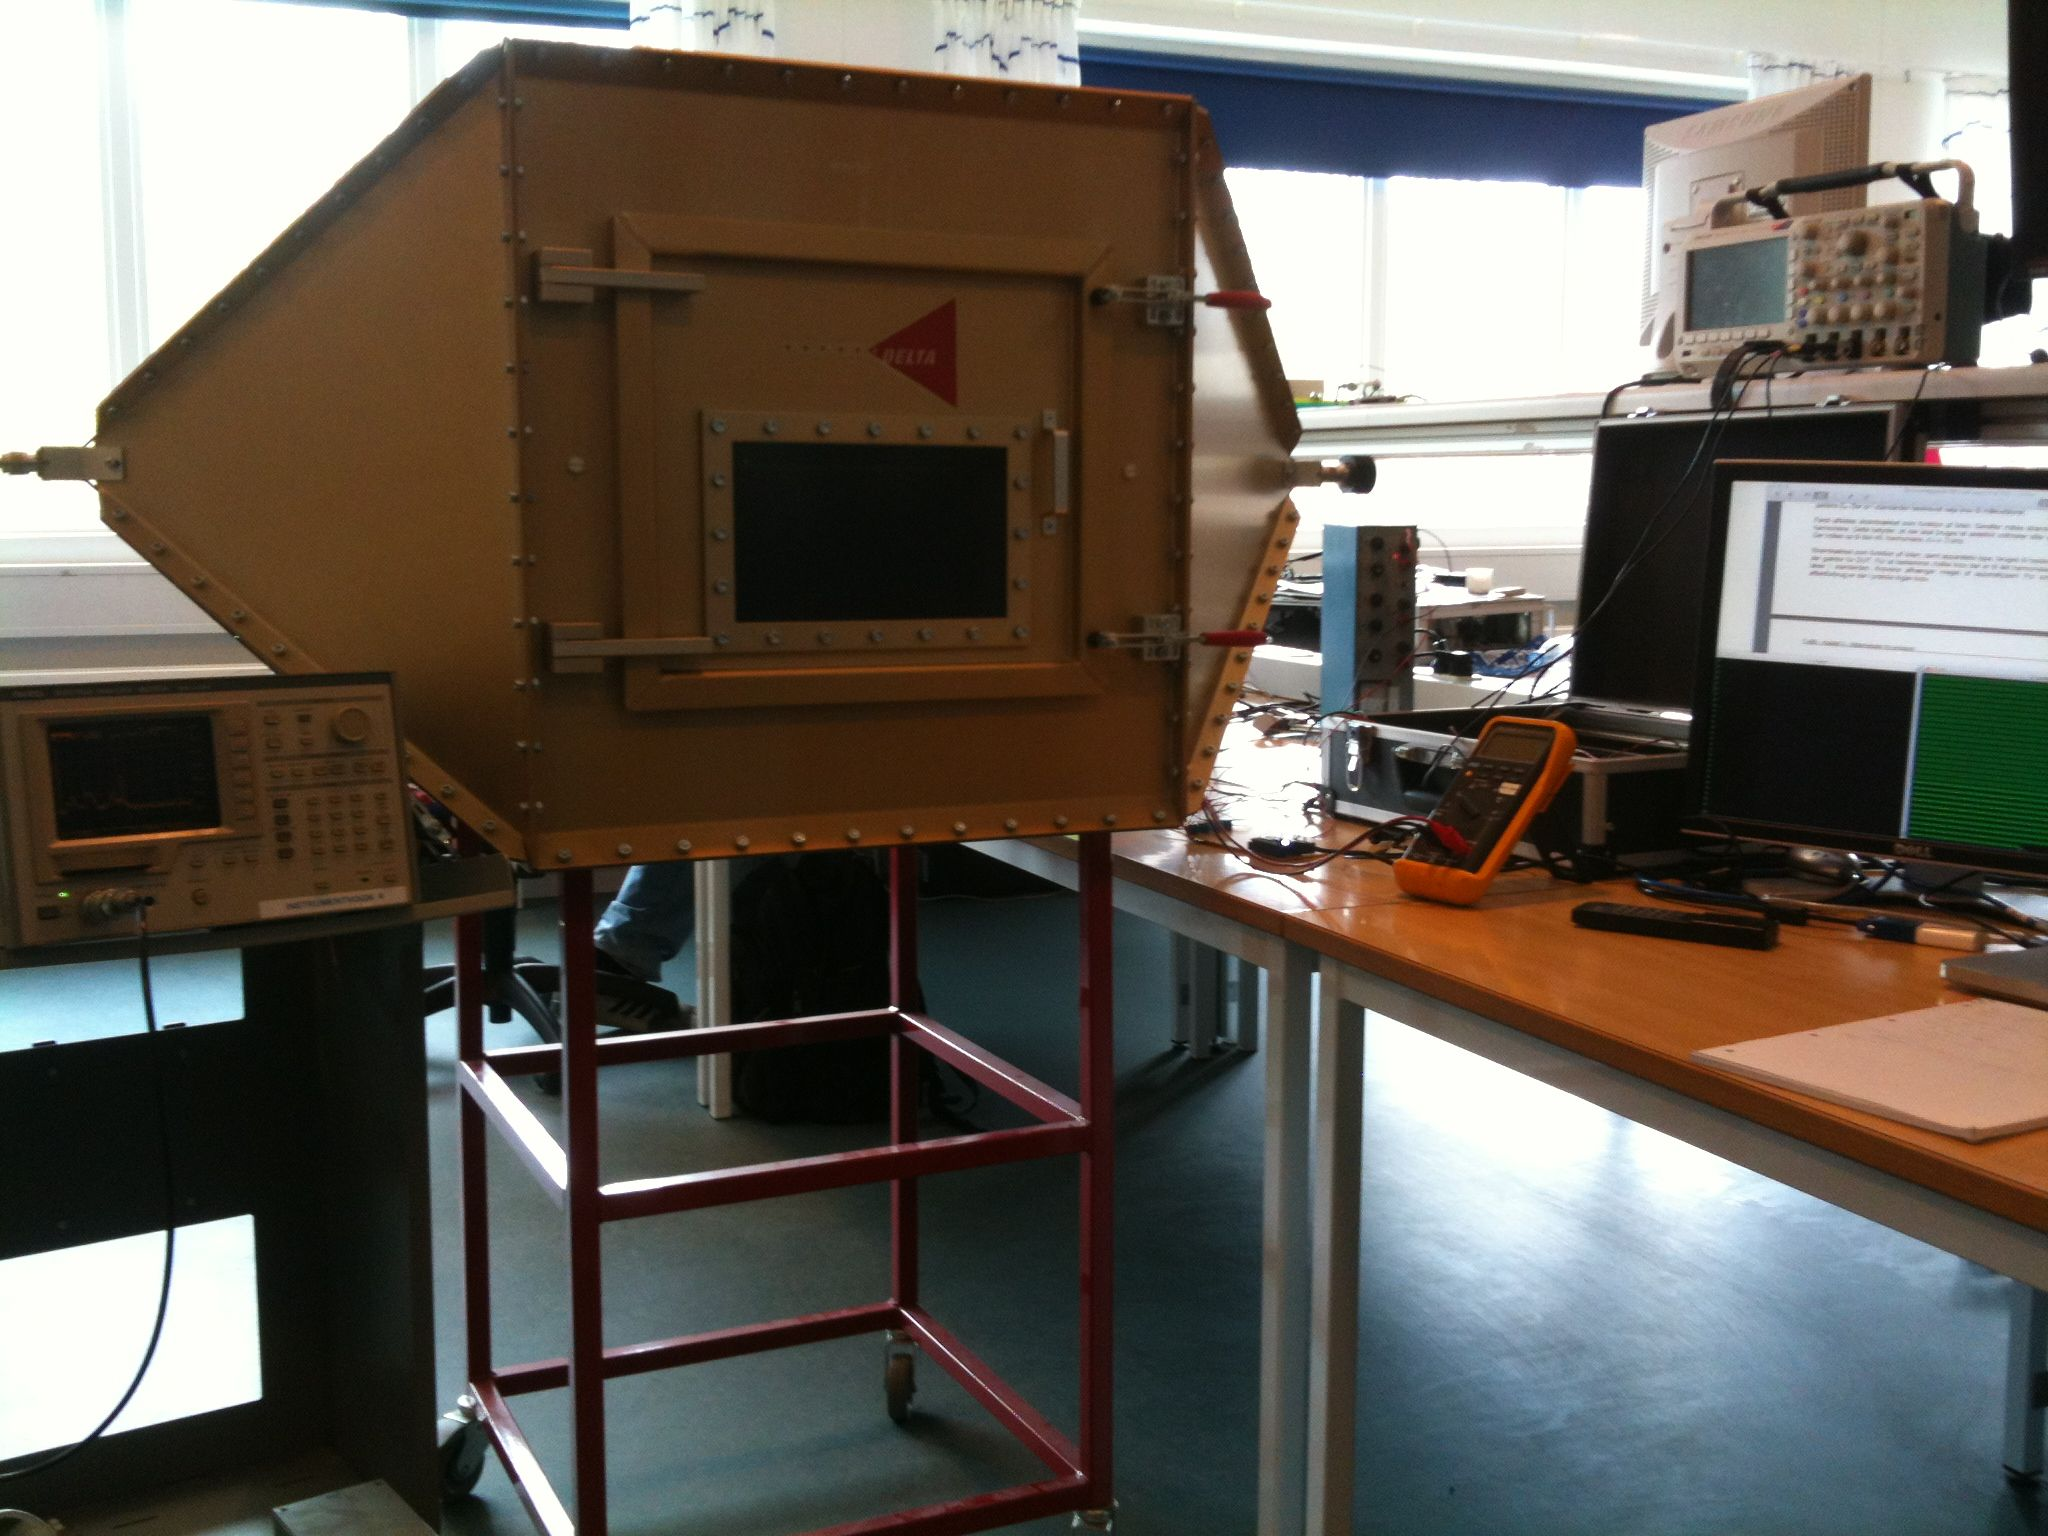
\includegraphics[width=0.8\textwidth]{images/tem_celle_radiation.jpg}
		\caption{Emission test setup.}
	\end{centering}
\end{figure}

\begin{figure}[H]
	\begin{centering}
		 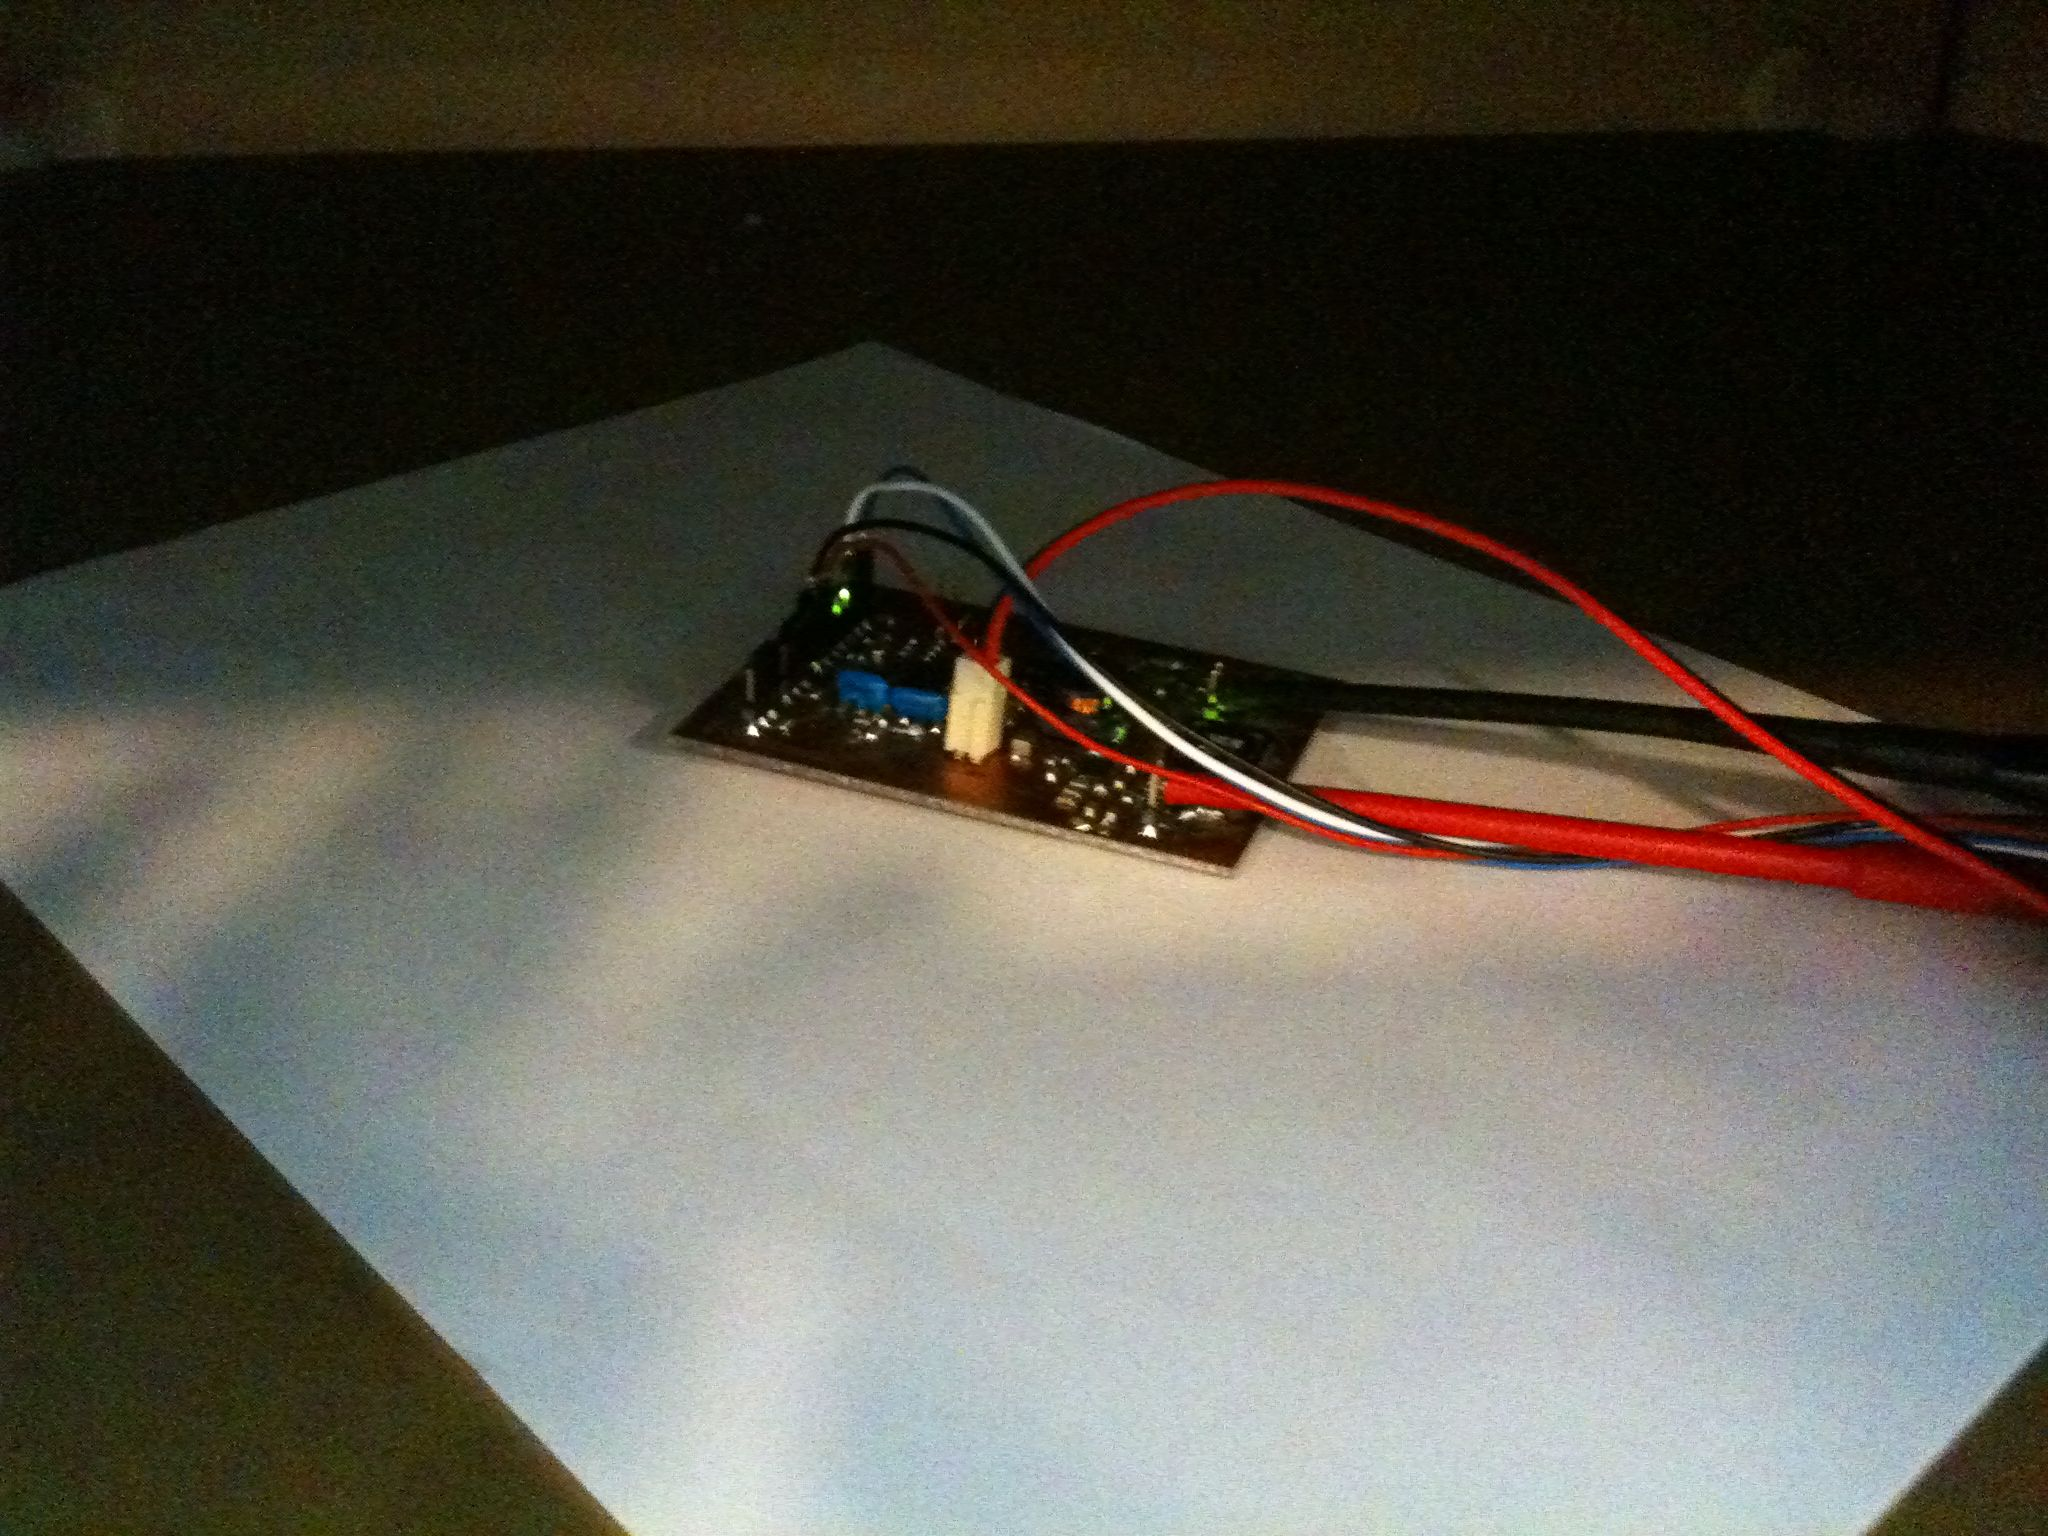
\includegraphics[width=0.6\textwidth]{images/board_placement.jpg}
		\caption{Board placement inside the TEM-cell.}
	\end{centering}
\end{figure}

\begin{figure}[H]
	\begin{centering}
		 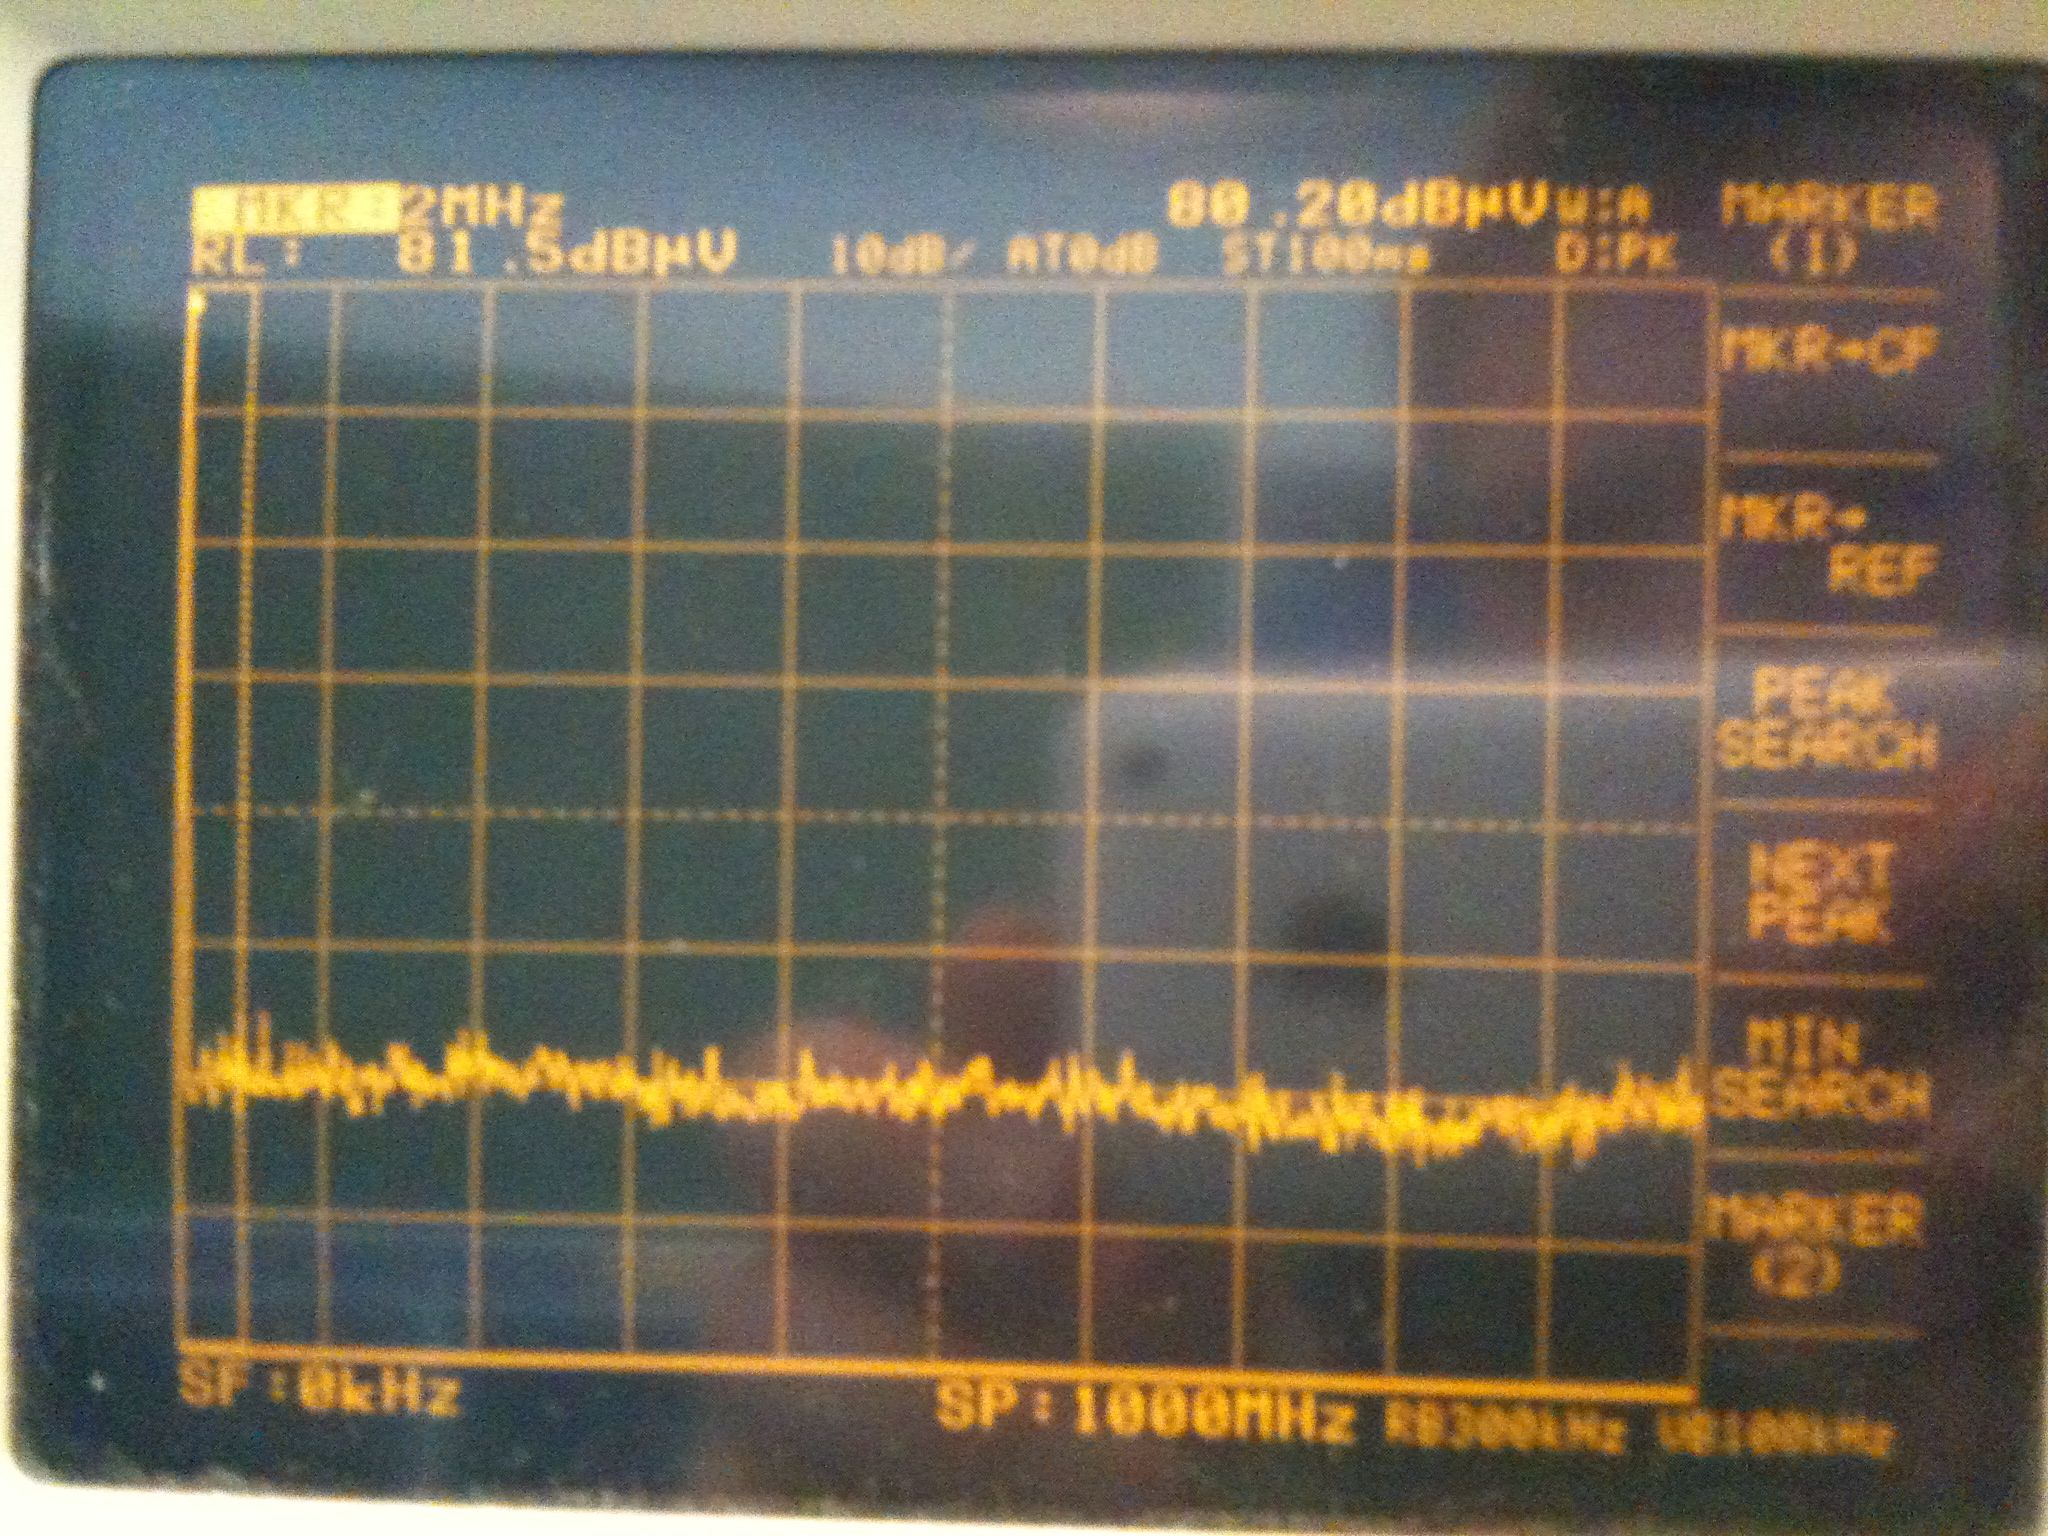
\includegraphics[width=0.6\textwidth]{images/measure_off.jpg}
		\caption{Spectrum analyzer when the device is turned off.}
	\end{centering}
\end{figure}

\begin{figure}[H]
	\begin{centering}
		 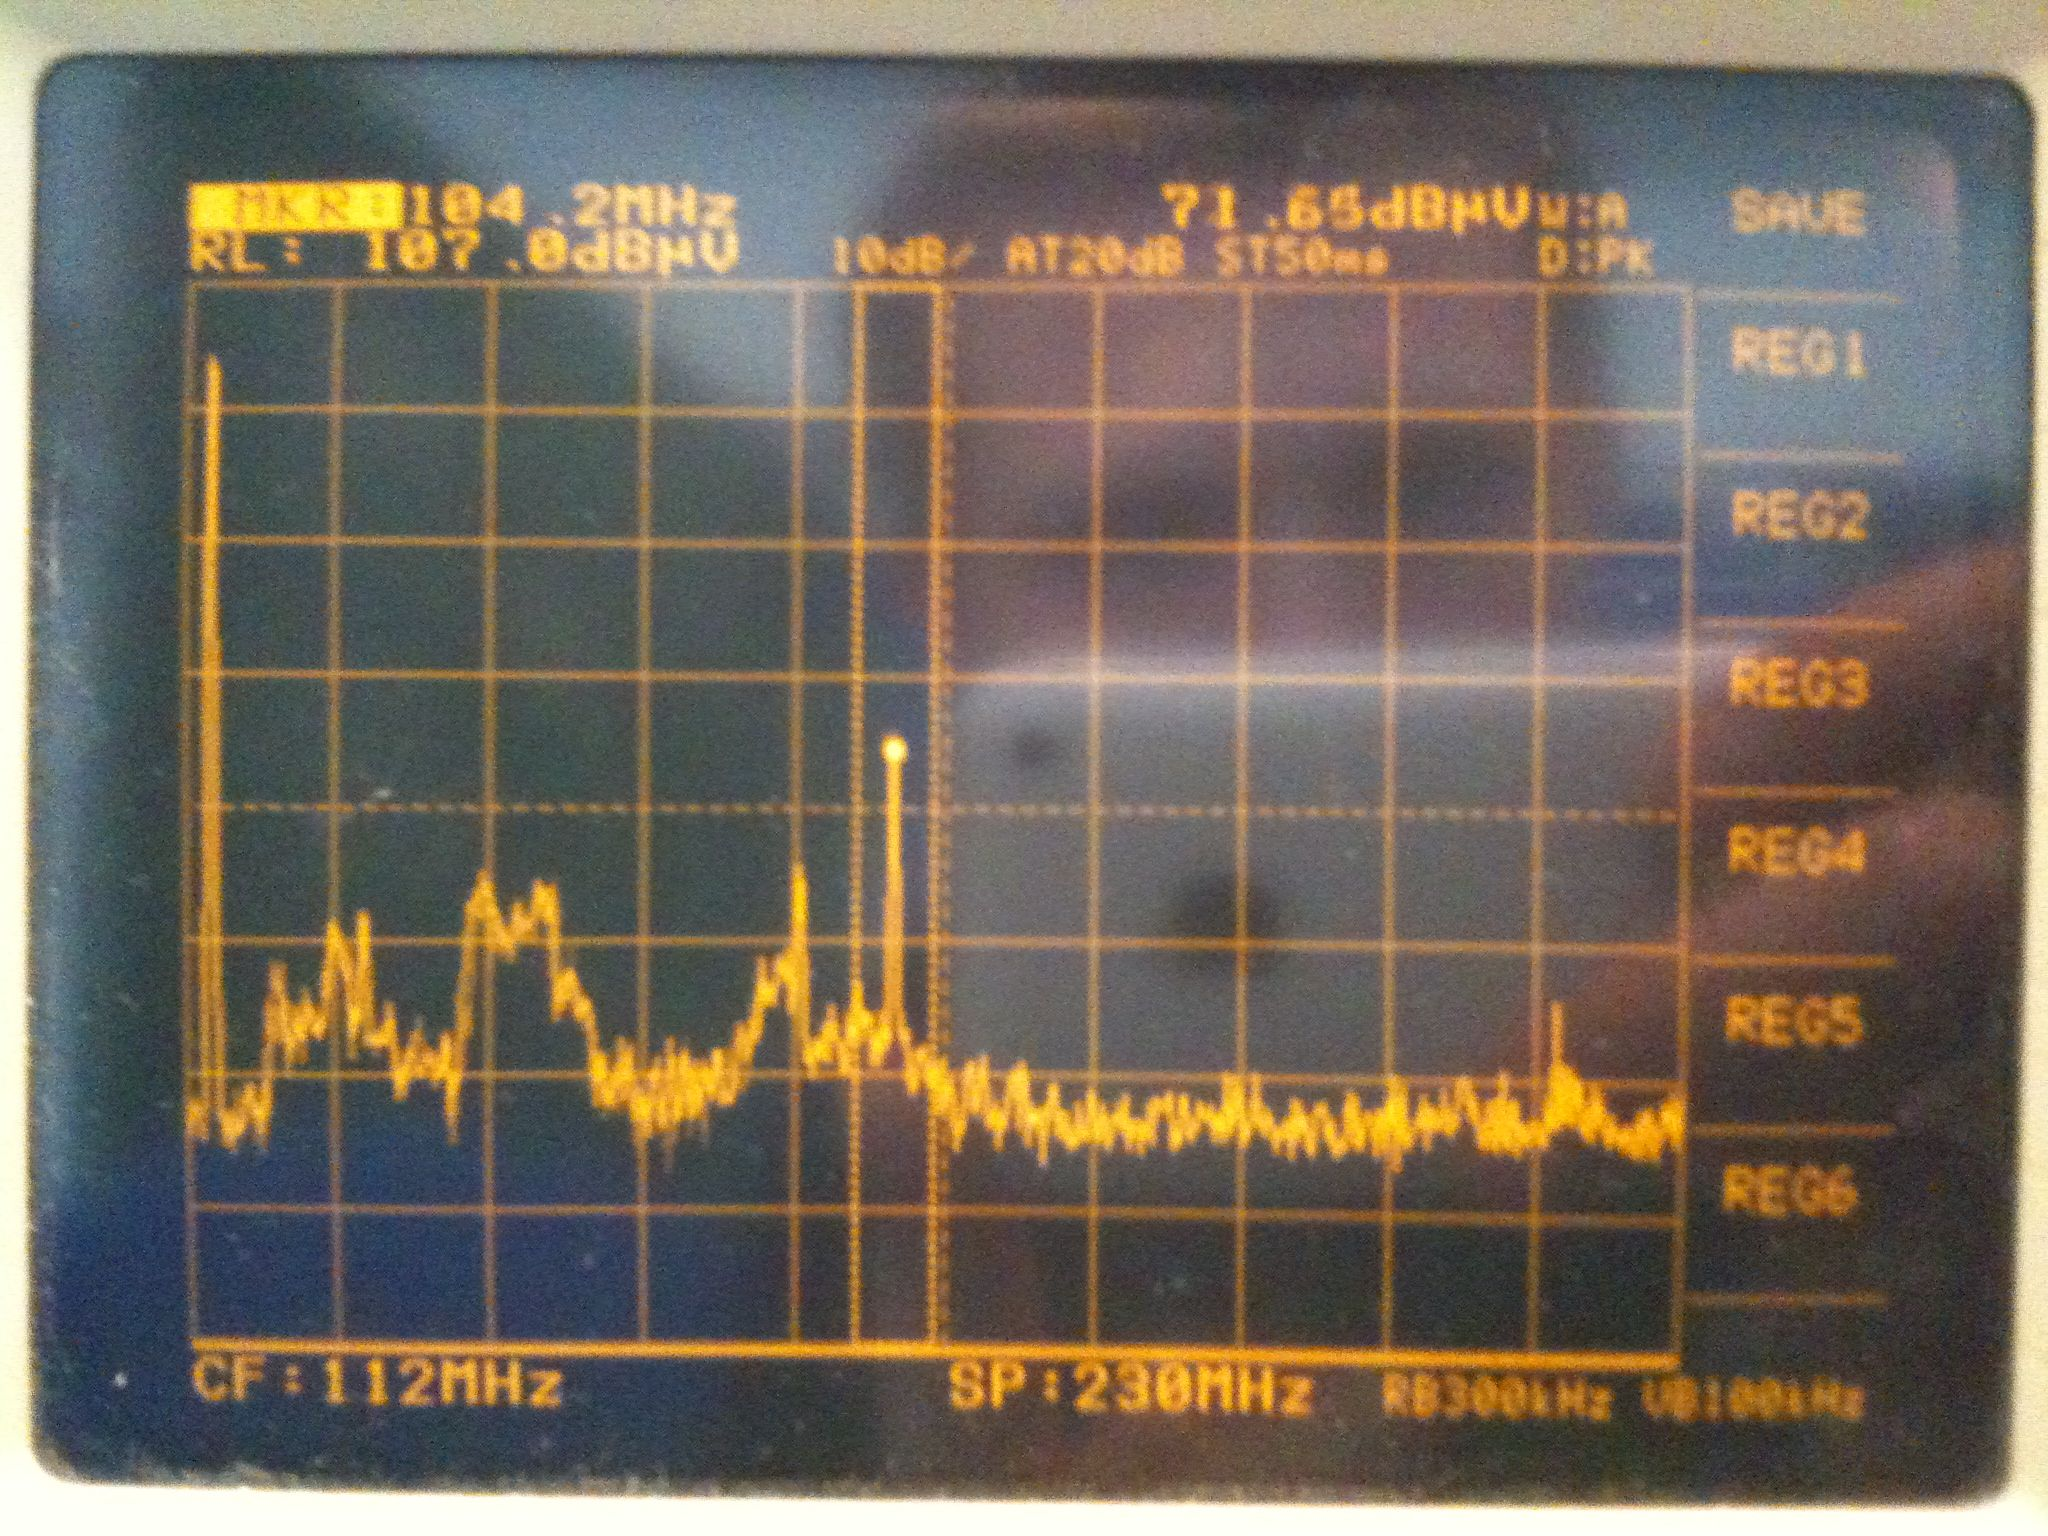
\includegraphics[width=0.8\textwidth]{images/measure_on.jpg}
		\caption{Emission spectrum of the unit.}
	\end{centering}
\end{figure}

\begin{figure}[H]
	\begin{centering}
		 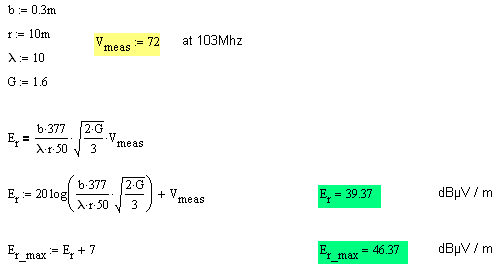
\includegraphics[width=0.8\textwidth]{images/mathcad_emission}
		\caption{MathCAD calculation of the emission.}
	\end{centering}
\end{figure}

\section{Immunity test}
Down below different test cases are described, which the product has to fulfill in order to be EMC proved and get the CE mark. Only two of the tests are performed as the other tests can be destructive to the product and we only have one board mounted for our use. Normally the board will also be placed in a box (preferable a metal box connected to ground) to decrease the points of electrostatic discharge. The tests performed are: LF magnetic field immunity and HF irradiation.


\subsection{LF magnetic field immunity}

\subsection{HF irradiation}
For business and light industry, EN61000-6-1, test level 3V/m
\\ Industrial environment, EN61000-6-2, test level 10V/m

\subsection{Electrostatic discharge}
The test method is based on a generator (ESD-pistol) where two different kinds of discharges is performed: air discharge and discharge by contact. 
\\ The standard describes test values for up to 15kV for air discharge and up to 8kV for discharge at contact.
\\ However, in many product standards the values 8kV and 4kV is used (EN61000-6-1 and -2).


\subsection{Burst and energy transients}
Not tested as the board is not designed to withstand this!


%EN 61000-6-2 Immunity standard
%EN 61000-6-3 Emmision standard
